\documentclass[11pt]{jarticle}
\title{Grasshopper Tutorial}
\date{Feb 2017}
\usepackage{amsmath,bm,amsthm,amssymb}
\usepackage{listings}
\usepackage{fullpage}
\usepackage{ascmac}
\usepackage[dvipdfmx]{graphicx} % support the \includegraphics command and options to include graphics in your pdf
\usepackage{here}
%\fontfamily{arial}\selectfont
\renewcommand{\rmdefault}{phv}
\begin{document}
\maketitle
%
\section{練習: Surfaceの再構築}
この章では、基礎的なComponentを使い、Surfaceの再構築の方法を学びます。
また、Ghpythonを用いたプログラミングで同じ機能を実現するやり方を学びます。

\noindent 本章で必要なファイル: 
\begin{itemize}
\item
[1. ]Rhinoモデル: turbine.3dm
\item
[2. ]GHファイル: remake\_surface.gh
\end{itemize}

\noindent Surface再構築の手順: 
\begin{itemize}
\item
[1. ]SurfaceからCurveを抽出します (Brep Edges)。
\item
[2. ]分割数を指定し、Curve上を通るPointデータを作成します (Divide Curve)。
\item
[3. ]そのPointデータを通るNURBS Curveを構築します (Interpolate)。
\item
[4. ]4つのNURBS CurveからSurfaceを構築します (Edge Surface)。
\end{itemize}
本章ではこの4つを順にやっていきます。
図~\ref{fig:all} が今回のスクリプトの全体図を示しています。
このスクリプトを使えば、図~\ref{fig:surface} のように要素数を自由に変化させてsurfaceの再構築が出来ます。
一つ一つのブロックがcomponentと呼ばれるものでそれぞれがinputとoutputを持っています。
それぞれのcomponentの左側にあるものがinputで、右側にあるものがoutputです。
それでは、このスクリプトを作るプロセスを順に追って見ましょう。
%
\begin{figure}[H]
  \centering
    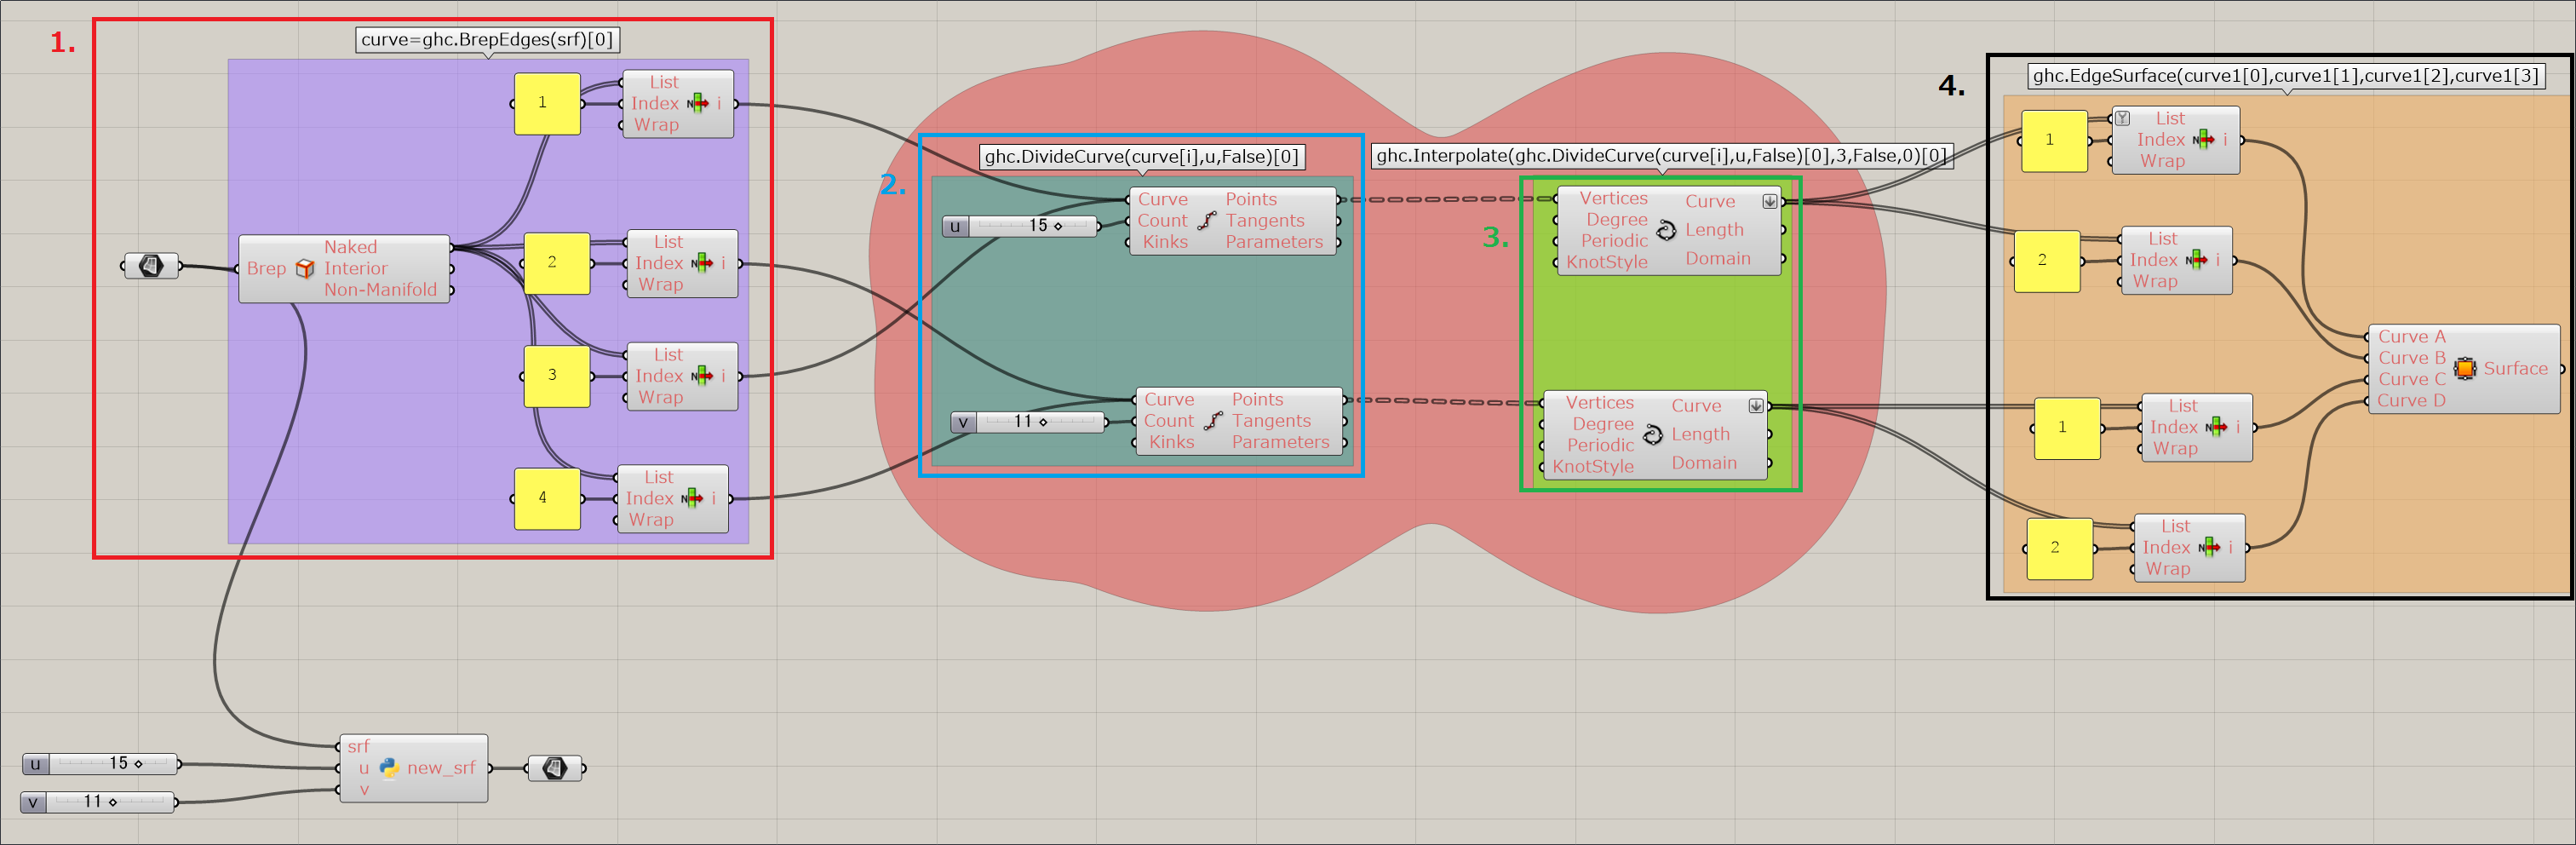
\includegraphics[width=\linewidth]{fig/gh_prog.png}
    \caption{全体像}
    \label{fig:all}
\end{figure}
%
\begin{figure}[H]
  \centering
    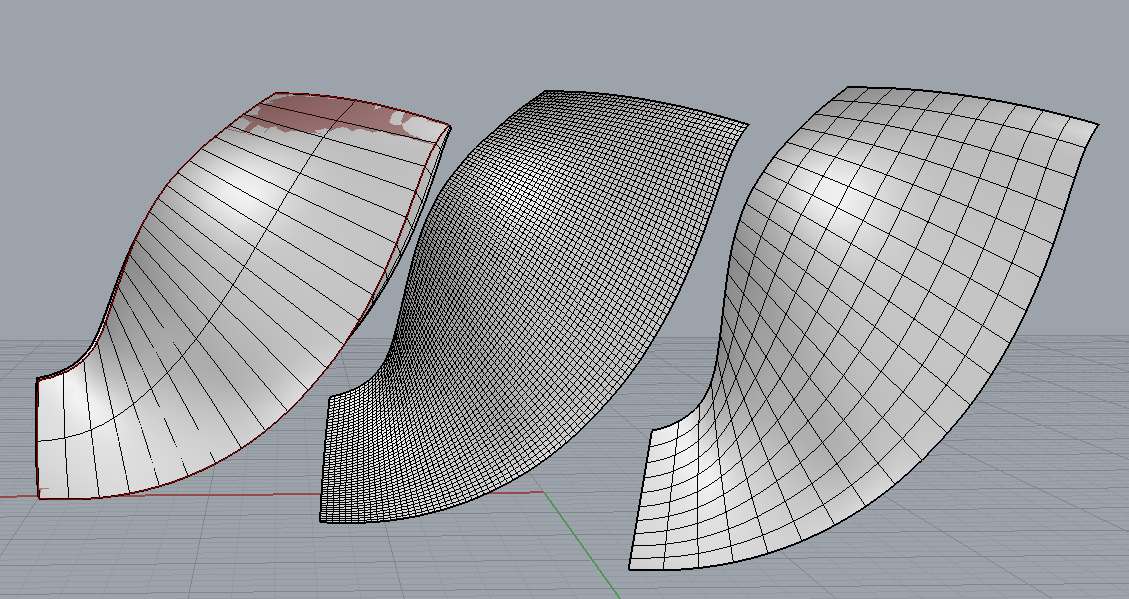
\includegraphics[width=\linewidth]{fig/finpng.png}
    \caption{Surfaceの要素数を変更できる}
    \label{fig:surface}
\end{figure}

\subsection{Componentを使って再構築する}
\subsubsection{SurfaceからCurveを抽出}
\label{sec:s1}
まず編集したいSurfaceをGrasshopperにパラメータとしてinputしなければいけません。
パラメータはすべてParamsのページでまとめており、Surfaceパラメータをキャンバスに配置します。\\
Params の中にも Geometry、Primitive、Specialの三種があります。\\
\begin{itemize}
\item
Geometry はインプットデータの取り込みができ、複数のコンポーネントに同じインプットデータ (線や平面) を用いるときに便利です。
\item
Primitive は数値などを扱うことができます。
\item
Special は数値を自由に変化させる slider やデータ (点集合の xyz など) を表示するなど、いろいろなことができます。
\end{itemize}
図~\ref{fig:setgeo} のように配置したSurfaceパラメータを右クリックするとコンテキストメニューが表示されるので、'Set one Surface'を選択します。
Rhinoceros内で指定したいSurfaceをクリックし、Surfaceパラメータがオレンジから白へと変化すれば、入力に成功です。

\begin{figure}[H]
  \centering
    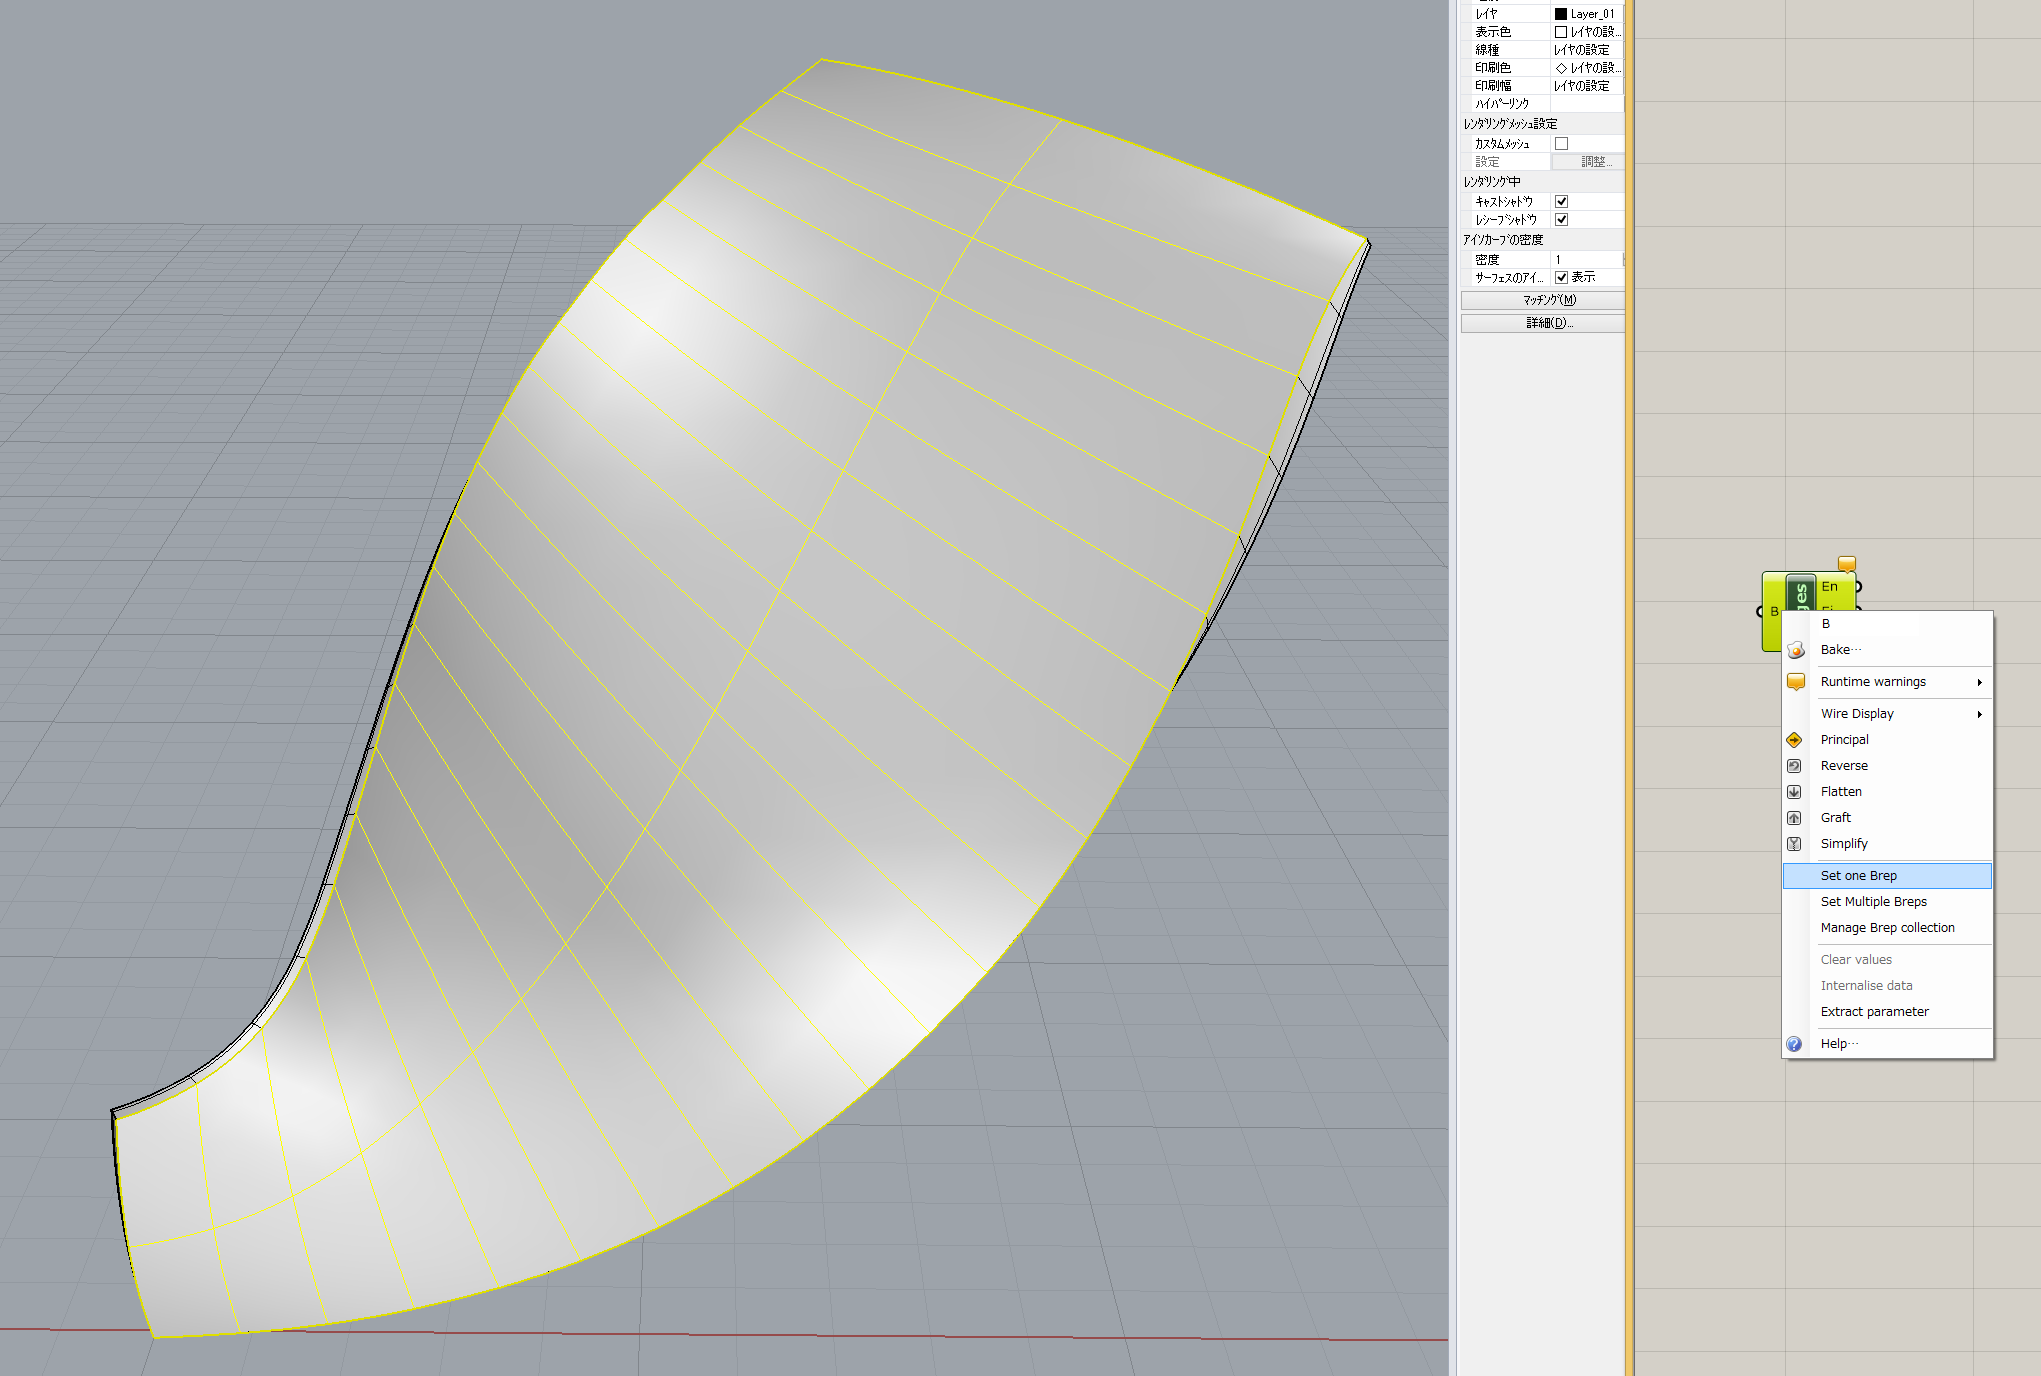
\includegraphics[width=\linewidth]{fig/setbrep.png}
    \caption{surfaceの選択}
    \label{fig:setgeo}
\end{figure}

\begin{itembox}[l]{Tip1: Componentがどこにあるのかを探したいとき:}
  Ctrl+Altを押して、マウスの右上にinformationマークが表示されたのを確認した後、componentを押すと、自動的にComponentのあるページと場所を矢印で示してくれます。
  各自ghファイルを開いてこの方法でチェックしてみてください (これ以降のComponentの場所は説明しません)
\end{itembox}

\begin{itembox}[l]{Tip2: Componentを挿入したいとき:}
  キャンパスの開いているところをダブルクリックすると、component検索ウインドウが出ます。componentの名前を入れると、上に表示するのでクリックしてキャンパスに配置します。\\
\begin{figure}[H]
\begin{minipage}{0.5\hsize}
\centering
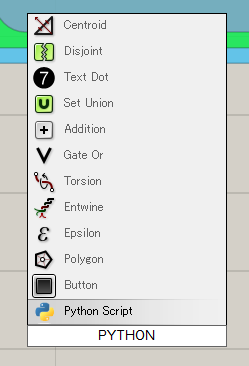
\includegraphics[width=\linewidth]{fig/python.png}
\caption{componentの検索}
\end{minipage}
\begin{minipage}{0.5\hsize}
\centering
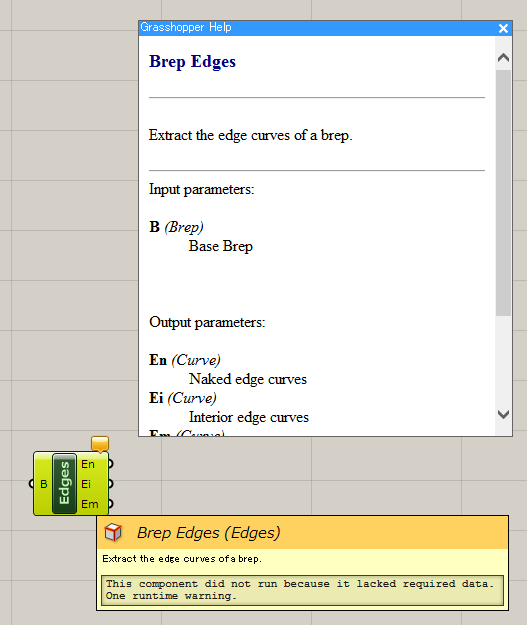
\includegraphics[width=\linewidth]{fig/brepedge_help.png}
\caption{componentのヘルプ}
\end{minipage}
\end{figure}
\end{itembox}

\begin{itembox}[l]{Tip3: Componentがどのような使い方をするのか調べたいとき:}
  Componentを代表している図形(または文字)を右クリックし、Helpを選択する。新しいComponentを使う前に必ず確認しましょう。
  同様にinputとoutputの入力形式を調べたいときは、カーソルを調べたものの上に右クリックしhelpを選択する。
\end{itembox}

\begin{itembox}[l]{Tip4: Input type}
  Componentに入力がある場合、Grasshopperは入力するデータタイプの認識ができないので、手動で設定する必要があります。
  Component上に接続する変数の名前のところを右クリックし、Data typeから適切なものを選びます。

\begin{figure}[H]
  \centering
    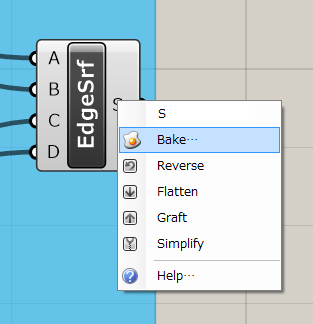
\includegraphics[width=0.8\linewidth]{fig/bake.png}
    \caption{bake}
  \label{fig:scanipflow}
\end{figure}

\end{itembox}
図~\ref{fig:components1} のように、Brep EdgesのComponentを配置し、inputを先ほどのSurfaceパラメータと接続します。
これによって、Surfaceのエッジ (4つのCurve) がひとつのListとして出力されます。\\
Listから要素を抽出するときは、List itemを使います。Listを入力し、Indexで要素番号を指定するとその要素が出力されます。
Indexの入力は、カーソルをindexの文字上において右クリック、'Set an integer'で数字を入れる方法。
または、何の数字を入れたのか後でわかりやすくできるように、Panel Componentを使用する方法があります。\\
\begin{figure}[H]
  \centering
    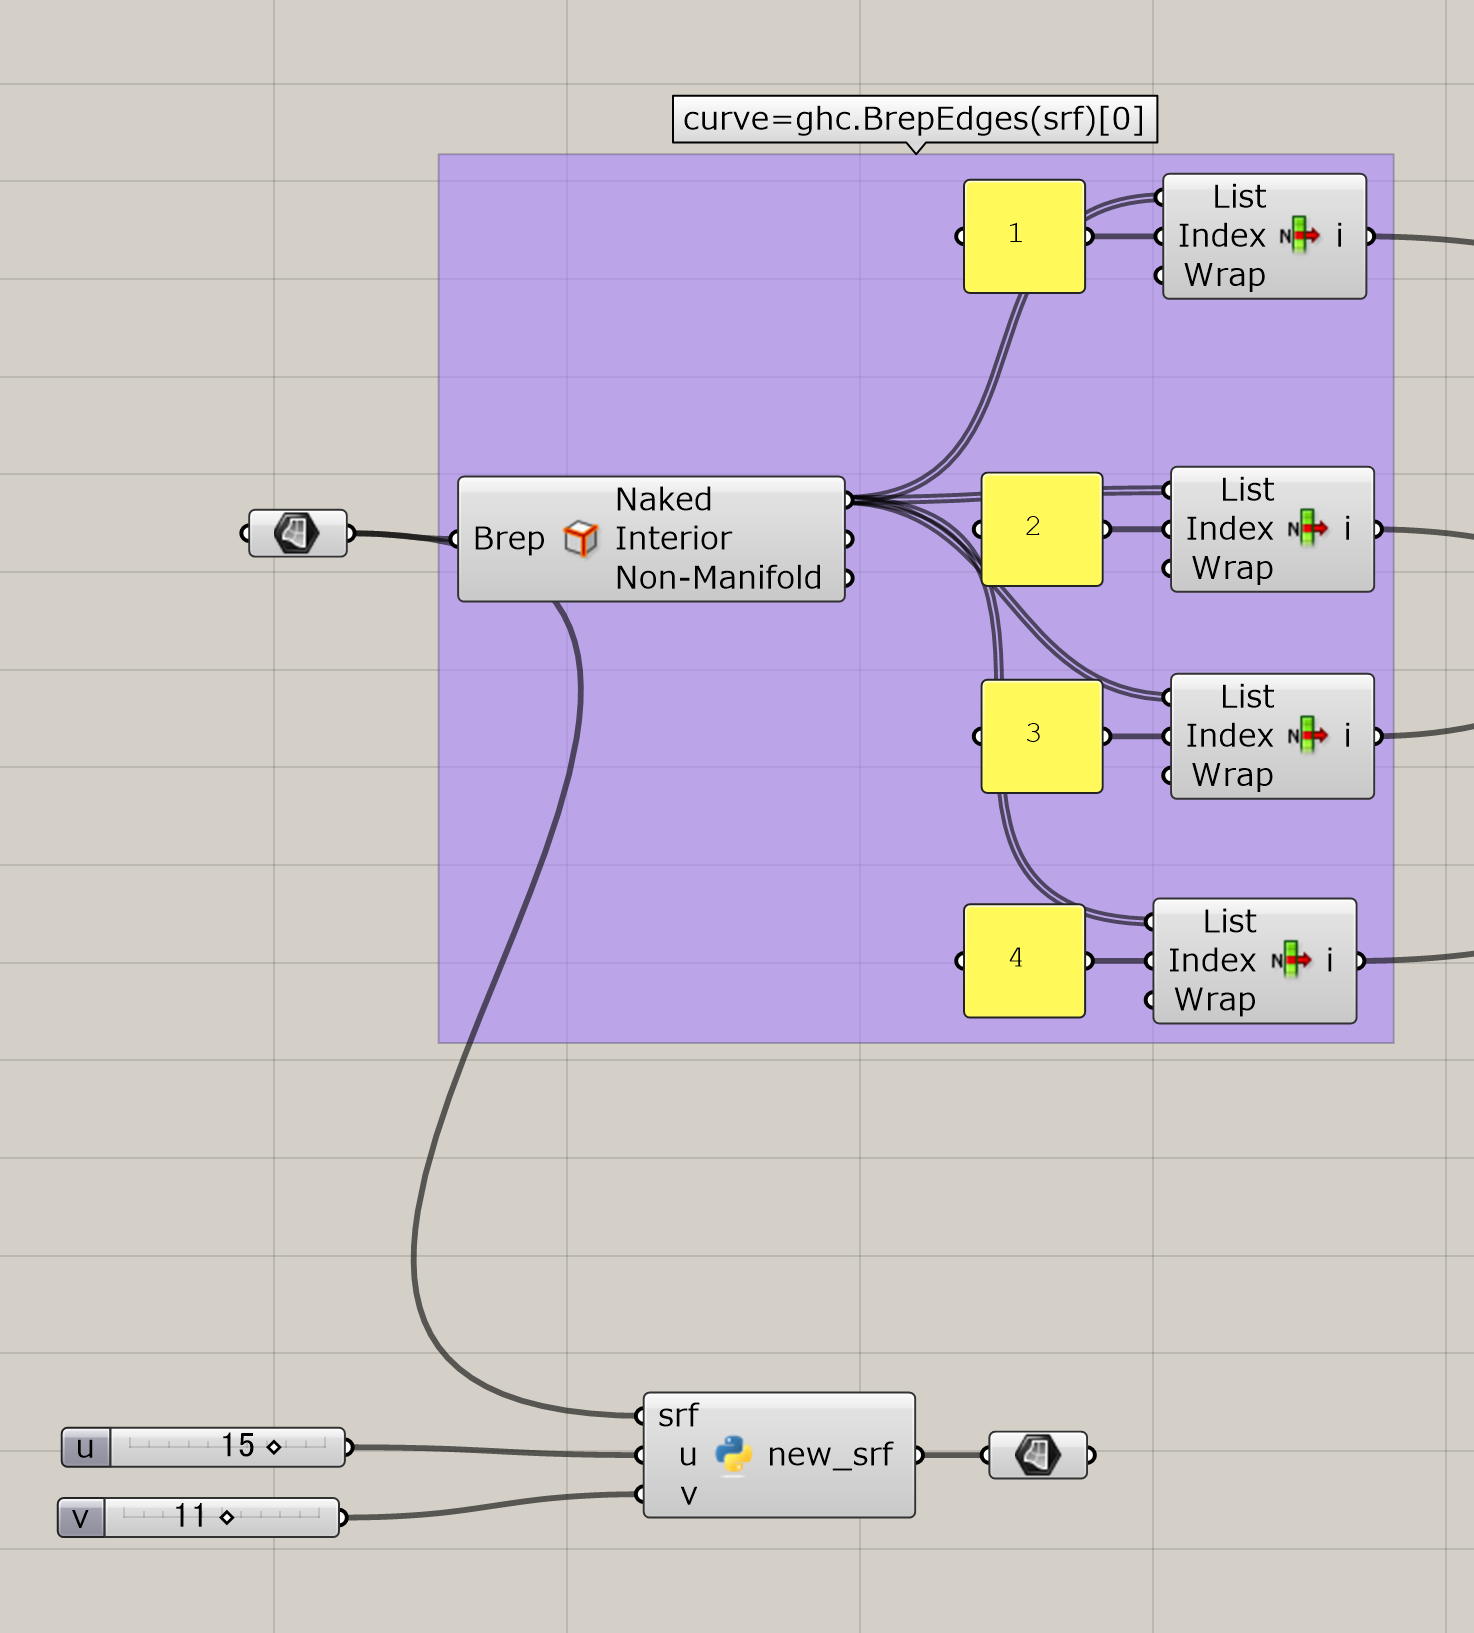
\includegraphics[width=0.7\linewidth]{fig/p1.png}
    \caption{\ref{sec:s1}節のcomponents}
    \label{fig:components1}
\end{figure}

\begin{figure}[H]
  \centering
    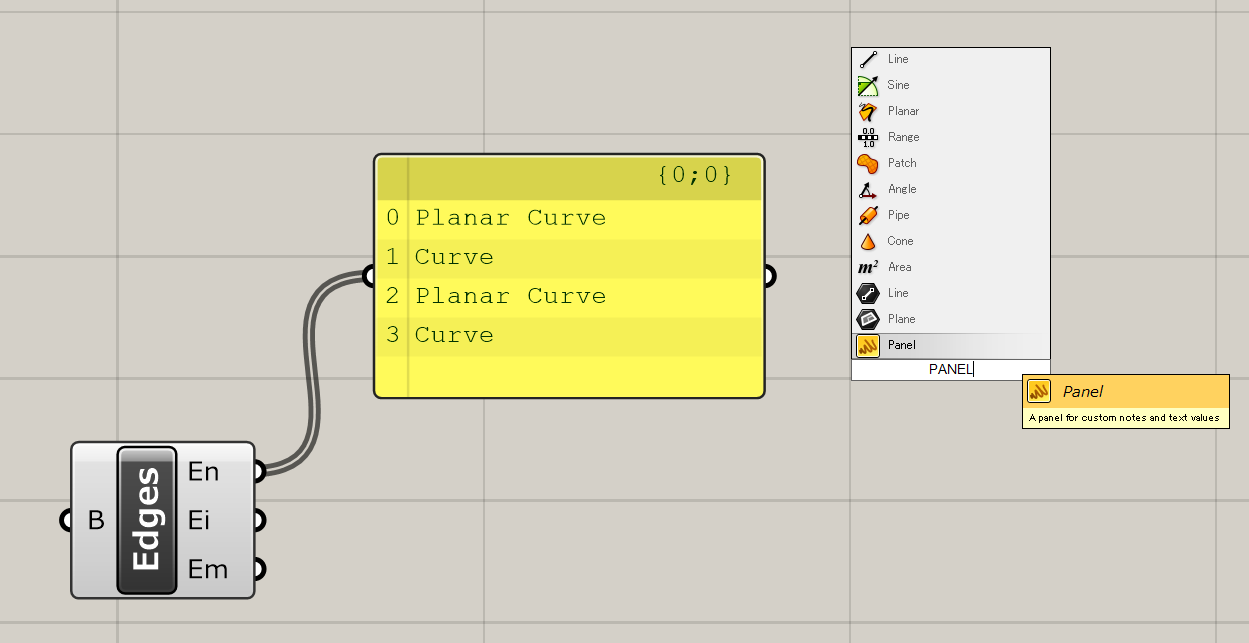
\includegraphics[width=0.5\linewidth]{fig/panel.png}
    \caption{Panelの挿入}
\end{figure}
\begin{itembox}[l]{Tip5:}
  データが一つの要素のとき、component同士をつなぐ線が実線になります。Listである場合は二重線、Tree Data (複数のList) である場合は点線となります。
\end{itembox}

\subsubsection{Curve上を通る点群を作成}
\label{sec:s2}
ここで使うComponent: Divede Curve\\
Divide Curveで分割数を指定し、分割点を出力してくれます。u,vの二方向があるので、二つDivide Curve Componentを配置します。\\
図\ref{fig:components2} のようにBrep Edges で出力されるCurveは時計回りに配置しているので、奇数番目のCurveをu方向、偶数番目のCurveをv方向にまとめて入力します。複数のデータを一つの場所に線を繋ぐときはshift押しながら線を繋ぎましょう。\\
Divide CurveのCount入力にSliderをつなぎます。
\begin{itembox}[l]{Tip6: Slider}
Sliderは型 (int、double) の指定、範囲 (Range) の指定をし、つまんで動かすことで、数値の変更に合わせたジオメトリの変化をリアルタイムで見ることができます。
型、範囲の指定は slider を右クリック、Edit でできます。
\end{itembox}

\label{sec:s2}
\begin{figure}[H]
  \centering
    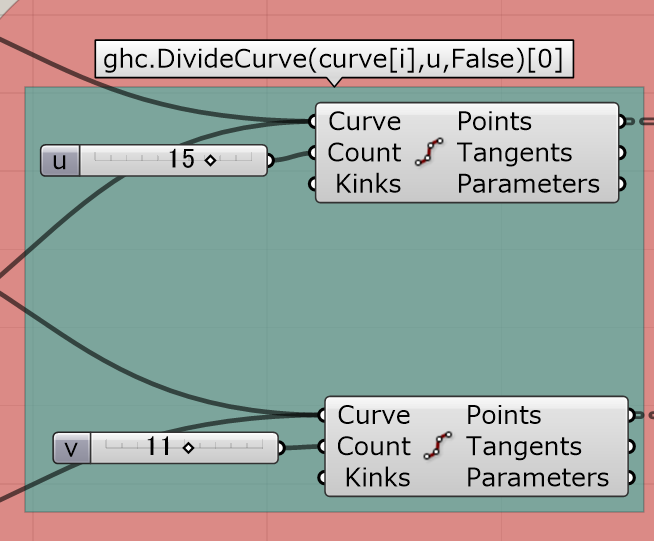
\includegraphics[width=0.7\linewidth]{fig/p2_1.png}
    \caption{\ref{sec:s2}節のcomponents}
    \label{fig:components2}
\end{figure}

\subsubsection{点群を通るNURBS Curveの構築}
\label{sec:s3}
ここで使うComponent: Interpolate\\
PointデータをInterpolate Componentに繋ぎます。Degree,Periodic,Knotstyleは入力がないとデフォルト値で入力されます。
Interpolateは入力されたPointデータでCurveを作成してくれるものです。
二つのListでPointデータを入力したので、出力も二つのListとなります。
出力されるすべての要素を一つのListに入れたいときは、出力される場所にカーソルを合わせ、右クリックして、Flattenを選択しましょう。

\begin{figure}[H]
  \centering
    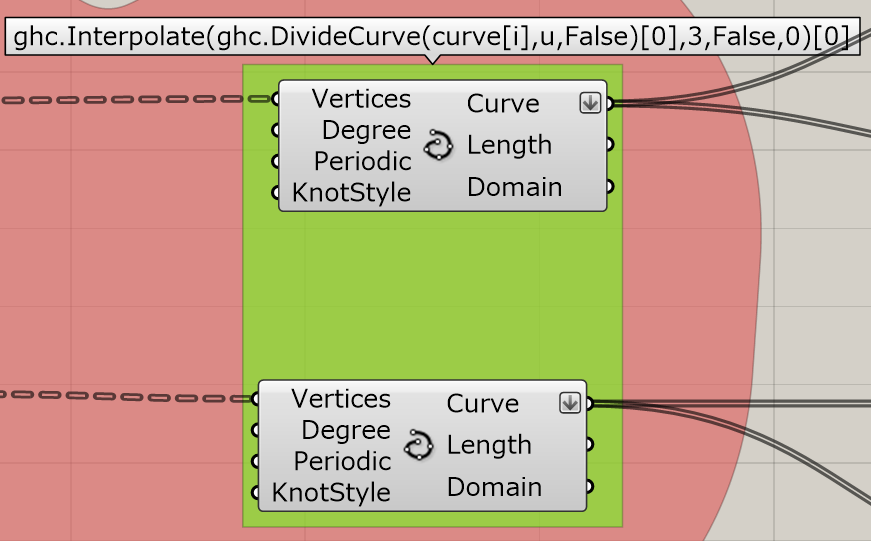
\includegraphics[width=0.7\linewidth]{fig/p2_2.png}
    \caption{\ref{sec:s3}節のcomponents}
    \label{fig:components3}
\end{figure}

\subsubsection{4つのNURBS CurveからSurfaceの構築}
\label{sec:s4}
\begin{figure}[H]
  \centering
    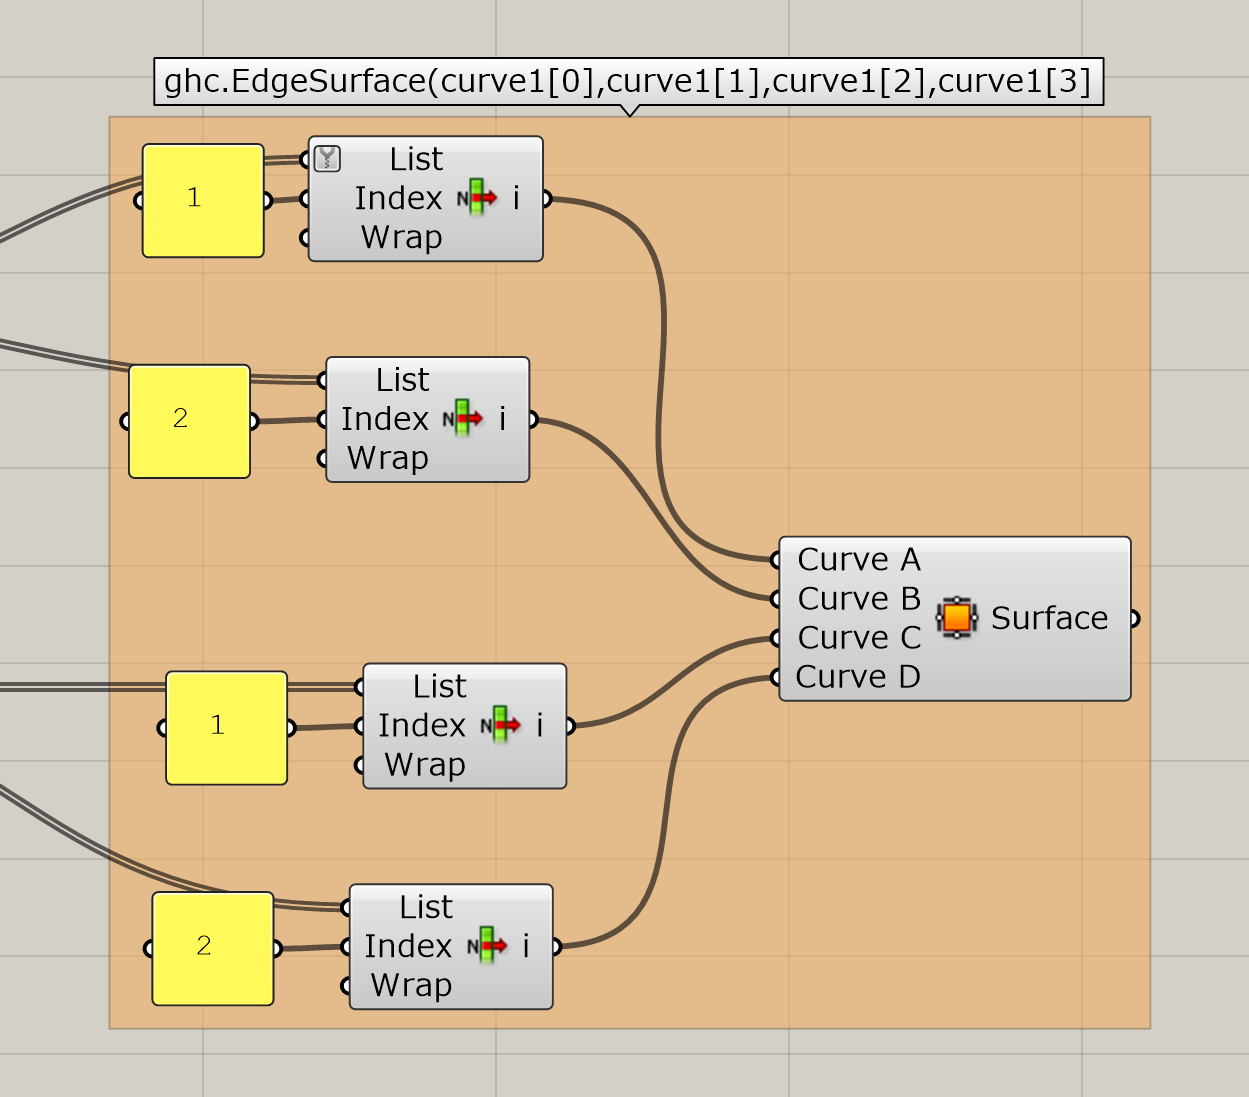
\includegraphics[width=0.7\linewidth]{fig/p3.png}
    \caption{\ref{sec:s4}節のcomponents}
    \label{fig:components4}
\end{figure}

ここで使うComponent: Edge Surface\\
Edge SurfaceはエッジであるCurveを入力すると、Surfaceを構築してくれるComponentです。
先ほどのInterpolateの出力は一つにつき、二つのCurveが入っているので、List itemでそれぞれ出します。
Edge Surfaceの出力を右クリック、Bakeを選択すれば完成です。

\begin{figure}[H]
  \centering
    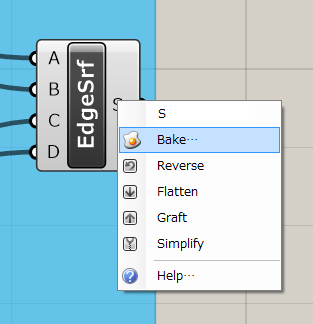
\includegraphics[width=0.6\linewidth]{fig/bake.png}
    \caption{Bakeのやり方}
  \label{fig:scanipflow}
\end{figure}
%
\subsection{Ghpythonによる作り方}
Ghpythonは、Grasshopper内でPythonによるプログラミングで図形の編集を可能としたツールです。
先ほどのプロセスと同じもので、プログラミングしたのが以下のコードとなります。
\begin{lstlisting}[basicstyle=\ttfamily\footnotesize]
import ghpythonlib.components as ghc
curve=ghc.BrepEdges(srf)[0]
curve1=[]
for i in range(0,4):
  if i\%2==0:
    curve1.append(ghc.Interpolate(ghc.DivideCurve(curve[i],u,False)[0],3,False,0)[0])
  else:
    curve1.append(ghc.Interpolate(ghc.DivideCurve(curve[i],v,False)[0],3,False,0)[0])    
new_srf=ghc.EdgeSurface(curve1[0],curve1[1],curve1[2],curve1[3])
\end{lstlisting}            

GrasshopperのComponentを使いたいときは、ghpythonlib.componentsを導入する必要があります。
\begin{lstlisting}[basicstyle=\ttfamily\footnotesize]
import ghpythonlib.components as ghc
\end{lstlisting}  

Componentを呼び出すときは、ghc.を打ち、その後にcomponentの名前をいれます。
\begin{lstlisting}[basicstyle=\ttfamily\footnotesize]
curve=ghc.BrepEdges(srf)[0]
\end{lstlisting}    
BrepEdgesは、三つの出力があります。Naked, Interior, Non-Manifold.
今回はNakedの出力が欲しいので、後ろに[0]をつけます。\\
Componentの正式な名前は、helpを調べたときに表示しています。
Ghpython内の各Componentの詳細な使い方は、ghc.component名を打ち終わったときに、code入力ウィンドウの下に自動的に表示します。\\
偶数番目のカーブをuとし、奇数番目のカーブをvとします。\\
\begin{lstlisting}[basicstyle=\ttfamily\footnotesize]
ghc.DivideCurve(curve[i],u,False)[0]
\end{lstlisting} 
がカーブを分割してポイントをアウトプットしています。その結果をInterpolateの入力として使います。
\begin{lstlisting}[basicstyle=\ttfamily\footnotesize]
ghc.Interpolate(ghc.DivideCurve(curve[i],u,False)[0],3,False,0)[0]
\end{lstlisting} 
そしてInerpolateして出来上がったカーブをcurve1というlistにappendします。
\begin{lstlisting}[basicstyle=\ttfamily\footnotesize]
curve1.append(ghc.Interpolate(ghc.DivideCurve(curve[i],u,False)[0],3,False,0)[0])
\end{lstlisting} 
四つのカーブがforで循環し終えた後、EdgeSurfaceを使って新しい面を作ります。
\begin{lstlisting}[basicstyle=\ttfamily\footnotesize]
new_srf=ghc.EdgeSurface(curve1[0],curve1[1],curve1[2],curve1[3])
\end{lstlisting} 
new\_surfをBakeすれば完成です。

\begin{figure}[H]
  \centering
    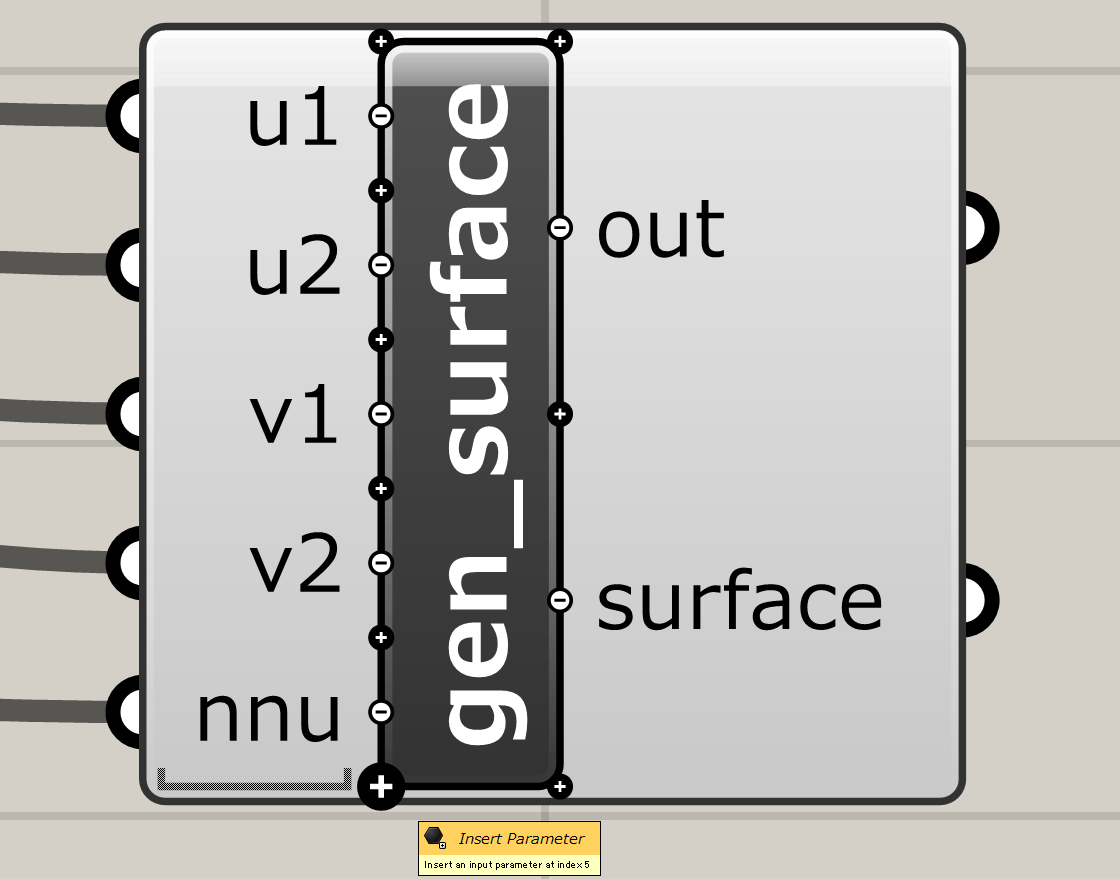
\includegraphics[width=0.8\linewidth]{fig/insert_parameter.png}
    \caption{Bakeのやり方}
  \label{fig:scanipflow}
\end{figure}
\end{document}
